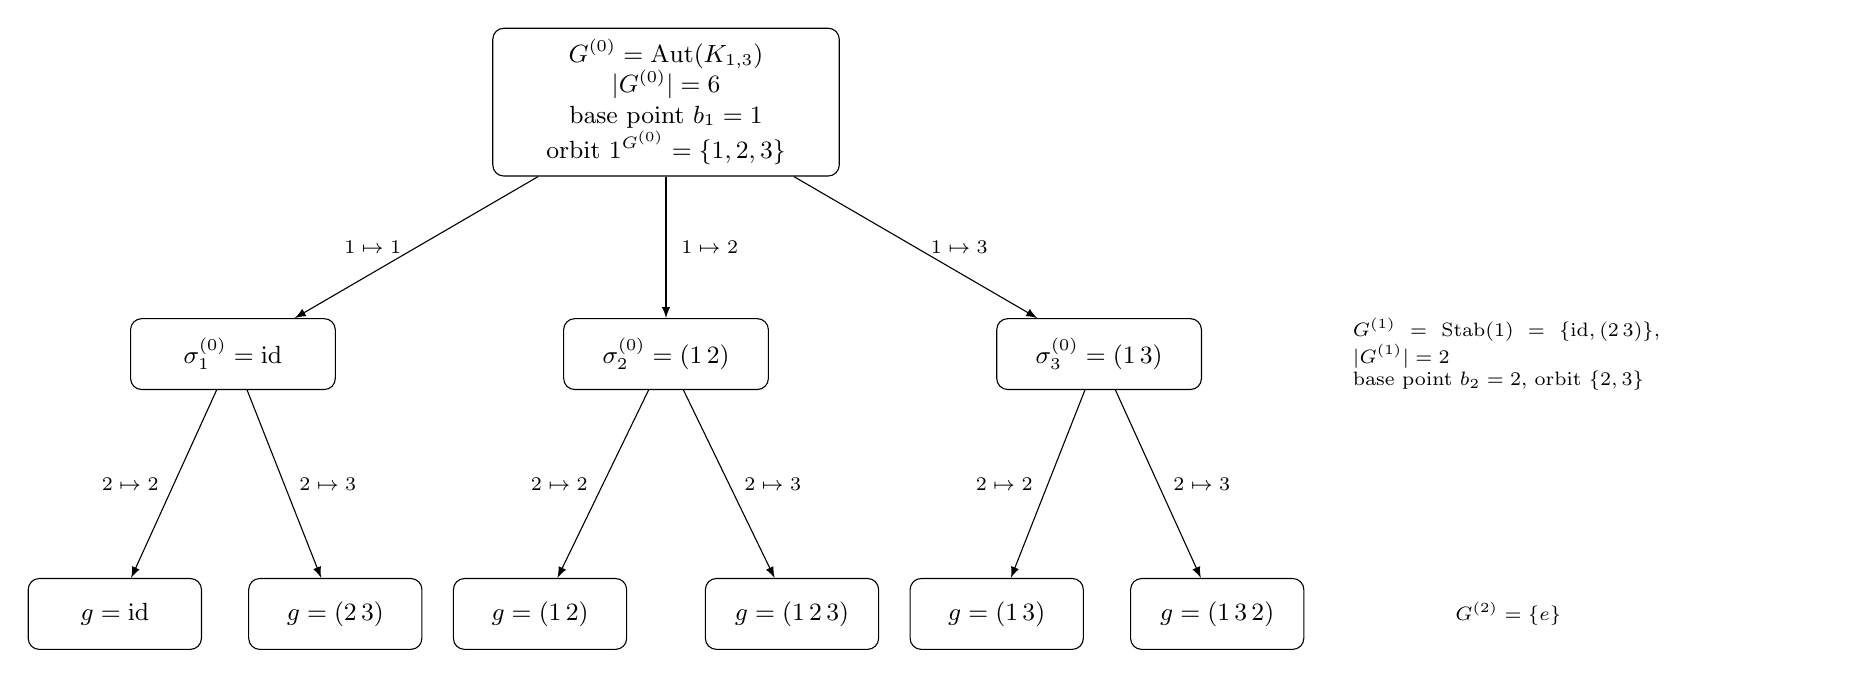
\begin{tikzpicture}[
  every node/.style={font=\small},
  level0/.style={draw, rounded corners, align=center, minimum width=4.4cm, minimum height=1.6cm, inner sep=4pt},
  level1/.style={draw, rounded corners, align=center, minimum width=2.6cm, minimum height=0.9cm, inner sep=3pt},
  leaf/.style={draw, rounded corners, align=center, minimum width=2.2cm, minimum height=0.9cm, inner sep=3pt},
  side/.style={align=left, font=\scriptsize, text width=4.6cm, anchor=west},
  >=latex
]

% --- Niveau 0 : G^{(0)} = Aut(K_{1,3}), |G^{(0)}|=6 ---
\node[level0] (root) at (0,7)
  {$G^{(0)} = \mathrm{Aut}(K_{1,3})$\\ $|G^{(0)}|=6$\\
   base point $b_1=1$\\ orbit $1^{G^{(0)}}=\{1,2,3\}$};

% --- Niveau 1 : trois cosets de G^{(1)} ---
\node[level1] (A) at (-5.5,3.8) {$\sigma^{(0)}_1=\mathrm{id}$};
\node[level1] (B) at (0,3.8)    {$\sigma^{(0)}_2=(1\,2)$};
\node[level1] (C) at (5.5,3.8)  {$\sigma^{(0)}_3=(1\,3)$};

\draw[->] (root) -- (A) node[pos=0.5, left=2pt]  {\scriptsize $1\mapsto1$};
\draw[->] (root) -- (B) node[pos=0.5, right=2pt] {\scriptsize $1\mapsto2$};
\draw[->] (root) -- (C) node[pos=0.5, right=2pt] {\scriptsize $1\mapsto3$};


\node[side] at (8.6,3.8)
{$G^{(1)}=\mathrm{Stab}(1)=\{\mathrm{id},(2\,3)\}$, $|G^{(1)}|=2$\\
 base point $b_2=2$, orbit $\{2,3\}$};

% --- Niveau 2 : les feuilles ---
\node[leaf] (A1) at (-7,0.5)   {$g=\mathrm{id}$};
\node[leaf] (A2) at (-4.2,0.5) {$g=(2\,3)$};
\node[leaf] (B1) at (-1.6,0.5) {$g=(1\,2)$};
\node[leaf] (B2) at (1.6,0.5)  {$g=(1\,2\,3)$};
\node[leaf] (C1) at (4.2,0.5)  {$g=(1\,3)$};
\node[leaf] (C2) at (7,0.5)    {$g=(1\,3\,2)$};

\draw[->] (A) -- (A1) node[pos=0.5, left=2pt]  {\scriptsize $2\mapsto2$};
\draw[->] (A) -- (A2) node[pos=0.5, right=2pt] {\scriptsize $2\mapsto3$};
\draw[->] (B) -- (B1) node[pos=0.5, left=2pt]  {\scriptsize $2\mapsto2$};
\draw[->] (B) -- (B2) node[pos=0.5, right=2pt] {\scriptsize $2\mapsto3$};
\draw[->] (C) -- (C1) node[pos=0.5, left=2pt]  {\scriptsize $2\mapsto2$};
\draw[->] (C) -- (C2) node[pos=0.5, right=2pt] {\scriptsize $2\mapsto3$};

% --- étiquette de niveau, à droite, alignée avec la rangée des feuilles ---
\node[side] at (9.9,0.5) {$G^{(2)}=\{e\}$};

\end{tikzpicture}